\documentclass[10pt,a4paper,notitlepage]{report}
\usepackage[utf8]{inputenc}
\usepackage[english]{babel}
\usepackage{amsmath}
\usepackage{amsfonts}
\usepackage{amssymb}
\usepackage{hyperref}
\usepackage{graphicx}
\usepackage{listings}
\usepackage{lmodern}
\usepackage{fourier}
\usepackage[left=2cm,right=2cm,top=2cm,bottom=2cm]{geometry}
\author{Steven Huerta}
\title{Pix ROS SITL Installation}
\begin{document}
\maketitle
\section*{Intro}
\noindent \textbf{DISCLAIMER:} This installation walkthrough and the software is owed to the hard work and efforts of the PX4 group (full citation below).\\

\noindent These instructions can be found at \hspace{2mm} \url{https://pixhawk.org/dev/ros/sitl}\\

\section*{LINUX INSTALL: Ubuntu 14.04}

\noindent \textbf{install-ros.bash}: Contains the installs for all the dependencies of the simulation.\\
\noindent \textbf{setup-workspace.bash}: Will create a workspace from the current directory for the simulation.\\

\noindent \textbf{IF YOU DO NOT WANT TO USE THE SCRIPTS}, you can copy and paste from the files to execute all or the portion of the script needed. The scripts do make life a bit easier.\\
\begin{enumerate}
\item Download the bash scripts found in this folder named \textit{install-ros.bash} and \textit{setup-workspace.bash}.
\item Make both files executable:
\begin{lstlisting}[language=bash]
$ chmod +x filename
\end{lstlisting}
\item Run both scripts sequentially. 
\begin{lstlisting}[language=bash]
$ ./install-ros.bash
$ ./setup-workspace.bash
\end{lstlisting}
\item You are done with the setup. You can begin using the simulation(Fig.~\ref{fig:sim}).
\end{enumerate}

\section*{Running the Simulation}

\begin{figure}[h]
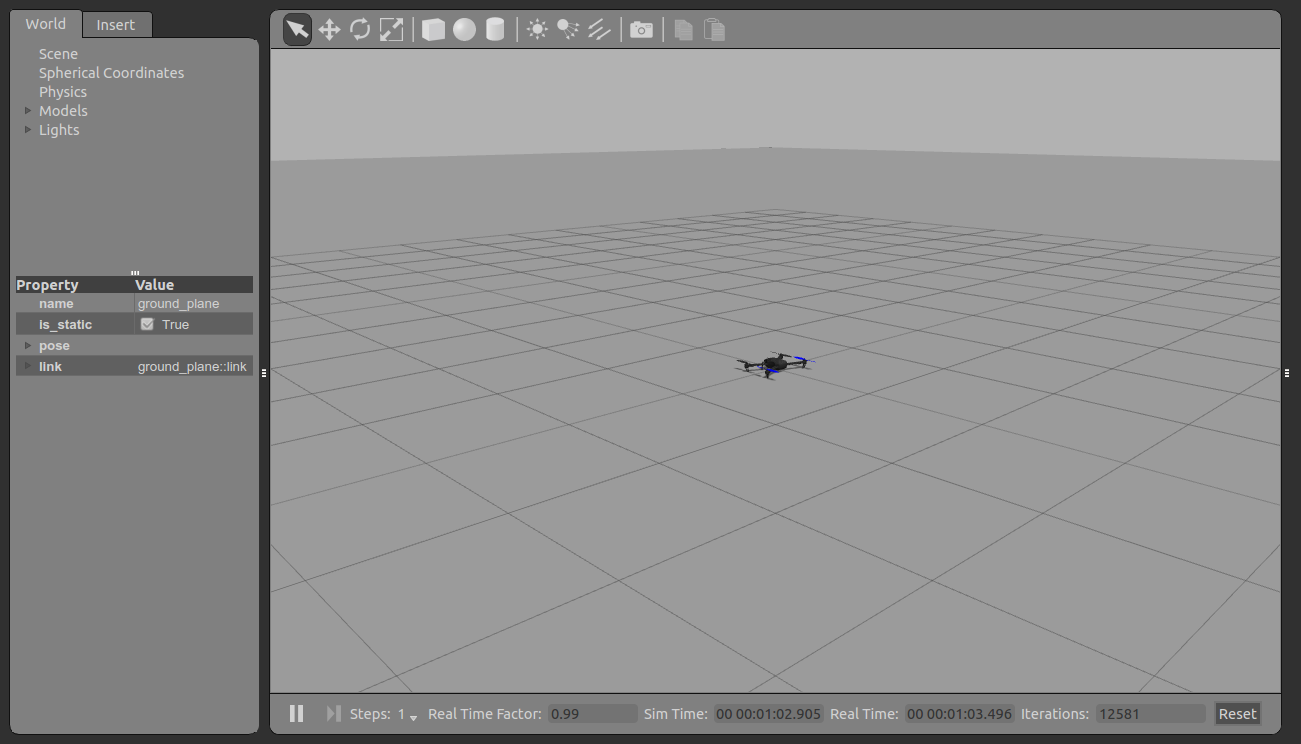
\includegraphics[width=4in]{rossitl.png}
\caption{UAV in Gazebo}
\label{fig:sim}
\end{figure}
\begin{enumerate}
\item Source the simulation
\begin{lstlisting}[language=bash]
your_workspace$ source devel/setup.bash 
\end{lstlisting}
\item Open a terminal and execute the script:
\begin{lstlisting}[language=bash]
your_workspace$ roslaunch px4 gazebo_iris_empty_world.launch 
\end{lstlisting}
\item At this point you can control the UAV manually using an XBox(or compatible) controller. We have found that other controllers are capable of controlling the craft, but the controls for steering and motor speed are mapped on the same stick.
\end{enumerate}


\noindent As a result of the flight controller being implemented using the ROS framework, the flight controller message traffic can be monitored using ROS tools(Fig.~\ref{fig:rostopics}), such as using:
\begin{lstlisting}[language=bash]
$ rosrun rqt_graph rqt_graph
\end{lstlisting}

\begin{figure}[h]
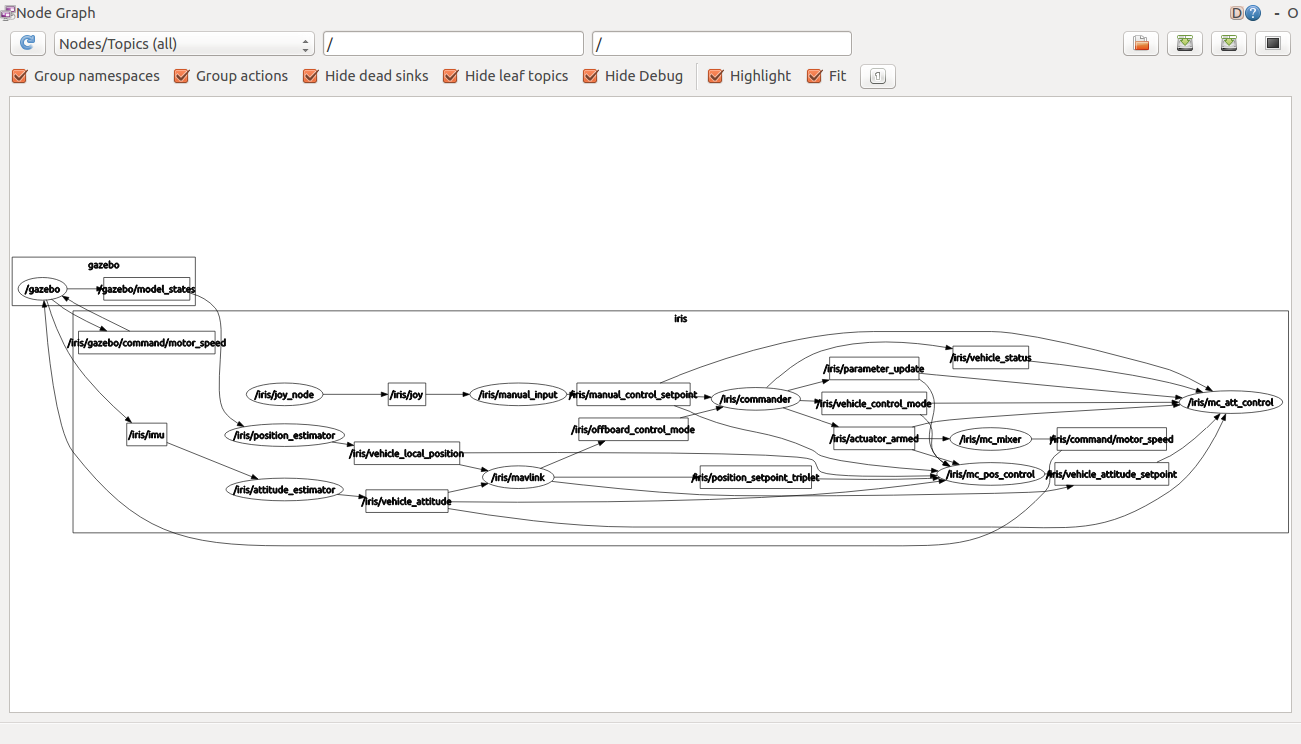
\includegraphics[scale=.35]{rqt_graph.png}
\caption{ROS Topic Publishers and Subscribers}
\label{fig:rostopics}
\end{figure}

\begin{thebibliography}{9}
\bibitem{lorenz} 
Lorenz Meier, Dominik Honegger and Marc Pollefeys. \textit{PX4: A Node-Based Multithreaded Open Source Robotics Framework for Deeply Embedded Platforms}, ICRA (Int. Conf. on Robotics and Automation) 2015.
\end{thebibliography}


\end{document}